With the two neural network architectures, the two loss function, our dataset and all the hyperparameters, we achieve to obtain result that we found good for our little dataset. 

\subsection{Hyperparameters}

To find the hyperparameters that gave the best images predictions on the test set, we did a grid search with a lot of check on the prediction by looking at the image. Our best result was achieve with the adapatation of the pretrained VGG 16. For the optimizer, we choose the stochastique gradient descent with a momentum of 0.9 and a small weight decay. The learning rate started at 0.001 and we decreased when the loss was not decreasing anymore. The batch size was 4, the dice loss was used, the image was normalize using the normalization of imagenet and we did 20 epochs. Here is the result that we gathered from our best experiments.
\vspace{2mm}
\setlength{\tabcolsep}{1mm}
\begin{tabular}{c c c c c}
	\toprule
	Model & Epochs & Loss & Train Loss & Valid Loss \\
	\midrule
	U-Net & 50 & Dice & 0.8263 & 0.8393 \\
	VGG16 & 20 & Dice & 0.8387 & 0.8023 \\
\end{tabular}

\vspace{1mm}

 The figure \ref{fig:test} is sample that shows our best results for VGG16 model on test set images.
 
 \begin{figure}[H]
 	\centering
 	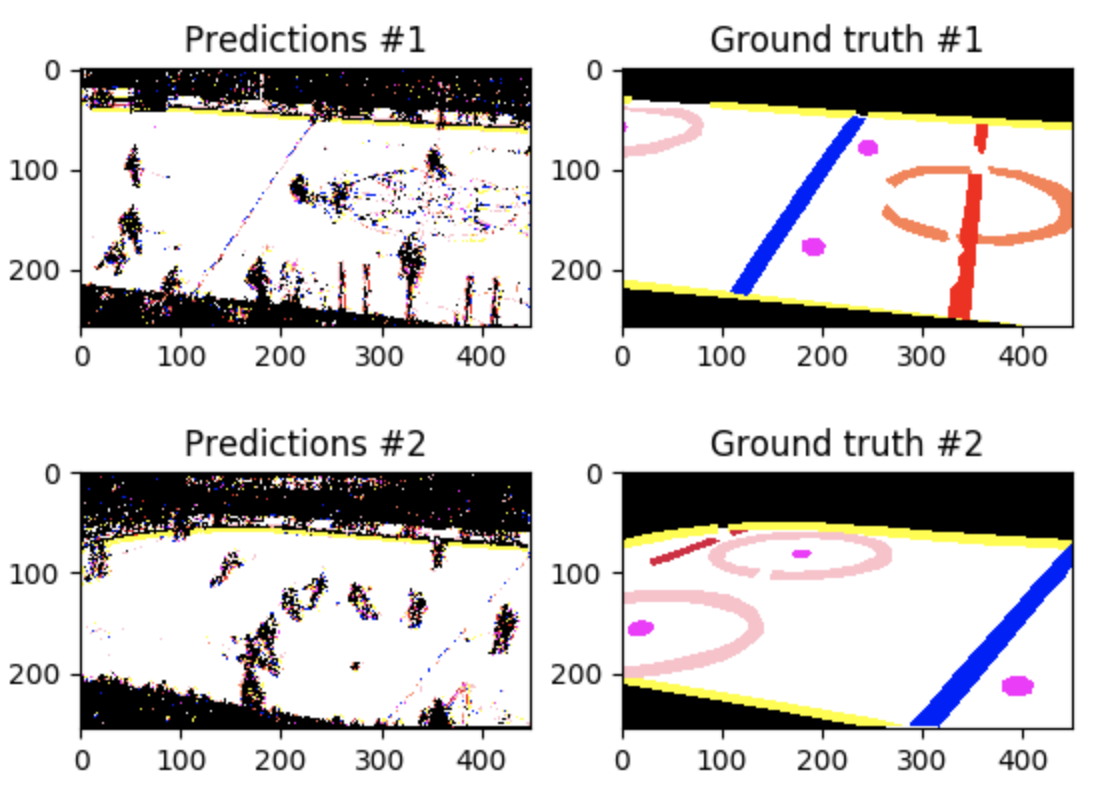
\includegraphics[width=7.5cm,height=4.86cm]{figures/test-9-class.png}
 	\caption{Sample of predictions of the VGG model on the test set.}
 	\label{fig:test}
 \end{figure}

We see that the upper board seems to be well predicted. The player on the ice are labelled as crowd, but it's not supprising since the player on the beach and the crowd are labbeled as crowd. The line appears a little bit.
